\section{Long-Term Dynamic Simulation Technique}
Time-sequenced power flow (TSPF) is a method for LTD simulation proven to generate useful results\cite{DonnellyVoltageControl}.
The basic idea behind TSPF is to solve a power flow, represent system dynamics of interest independent of the power flow solver, `re-seed' the power flow with new values, and repeat.
%While this task is monotonous for humans, it is well suited for computers.
A python based simulation software, Power System Long-Term Dynamic Simulator (PSLTDSim), has been developed to perform LTD simulations using TSPF.
PSLTDSim has the ability to calculate system frequency, perform governor dynamics, model automatic generation control (AGC), and insert step, ramp, and noise type perturbances into a power system.

%-------------------------------------------------------------------------------------
\subsection{Simulation Assumptions and Simplifications}
Due to the relatively large time steps of 1 second used with TSPF, numerous assumptions can be made.
Ideal exciters were assumed as modern exicters are typically fast enough to maintain reference voltage under stable conditions.
Intermachine oscillations were ignored since the time resolution used is not fine enough to capture these phenomena.

Simplifications of transient stability models are used in PSLTDSim.
The only parameters required to model a generator are the machine's rated MW, the machine's MVA base, and machine inertia.
Additionally, a deadband modified tgov1 governor model, Fig. \ref{fig: tgov1BlockDiagram},  was created to model system governors.

\begin{figure}[!ht]
	\centering
	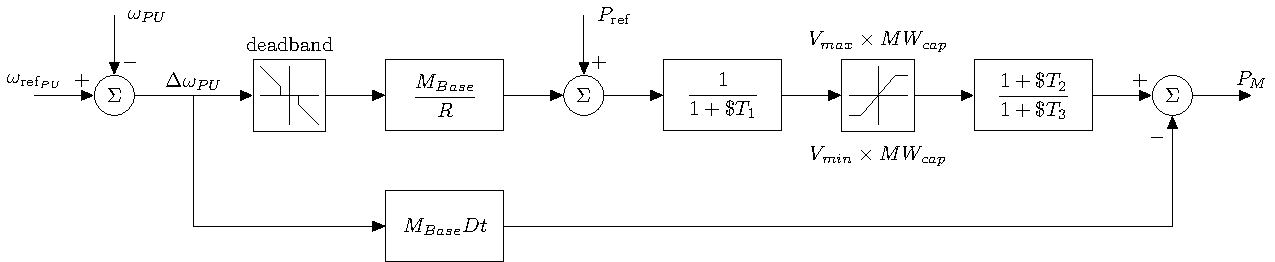
\includegraphics[width=\linewidth]{figures/tgov1DB}
	\caption{Block diagram of modified tgov1 model.}
	\label{fig: tgov1BlockDiagram}
\end{figure}

%-------------------------------------------------------------------------------------
\subsection{Modeling the System-Wide Frequency Response}
Instead of frequency being calculated for every bus, a combined swing equation is used to model only one system frequency.
As shown in (\ref{eq: CombinedSwingEq}), accelerating power from the entire system, as well as total system inertia $H_{PU, sys}$, is used to calculate $\dot{\omega}_{sys}$.

\begin{align}
\dot{\omega}_{sys} = \dfrac{1}{2H_{PU, sys} } \left( \dfrac{P_{acc PU, sys} }{\omega_{sys}} - D_{sys}\Delta\omega_{sys}  \right) \label{eq: CombinedSwingEq}
\end{align} 

%-------------------------------------------------------------------------------------
\subsection{Distribution of Accelerating Power}
In a system with $N$ generators, total system accelerating power is calculated by
\begin{align}
P_{acc, sys} = \sum_{i=1}^{N} P_{m,i}  - \sum_{i=1}^{N} P_{e,i} \label{eq:Pacc} 
\end{align}
\noindent where $P_{m,i}$ is mechanical power and $P_{e,i}$ is electrical power of generator $i$.

System accelerating power is distributed to all generators in the system according to machine inertia as
\begin{align}
P_{e, i} = P_{e, i}  - P_{acc, sys}\left( \dfrac{H_i}{H_{sys}}\right) \label{eq:distPacc}
\end{align}
where $H$ has units of $MW\cdot s$.

The new value for $P_{e, i}$ is used in the next power flow solution for each generator.
%Once all accelerating power is distributed, the new value for each generators power output is used as initial conditions to solve a power flow. 
If the difference between expected and resulting power supplied by the slack generator is larger than a set slack tolerance, the difference is redistributed according to (\ref{eq:distPacc}) until the resulting difference is below the slack tolerance, or a maximum number of iterations take place\cite{Stajcar}.
% should probably cite stajcar
